\documentclass[tikz,border=8pt]{standalone}
\usepackage{lmodern}
\usepackage{pgfplots}
\usepgfplotslibrary{groupplots}
\pgfplotsset{compat=1.18}
\definecolor{ink}{HTML}{183B4E}
\definecolor{teal}{HTML}{168C8C}
\definecolor{gold}{HTML}{D9982F}
\definecolor{violet}{HTML}{7B61A8}
\begin{document}
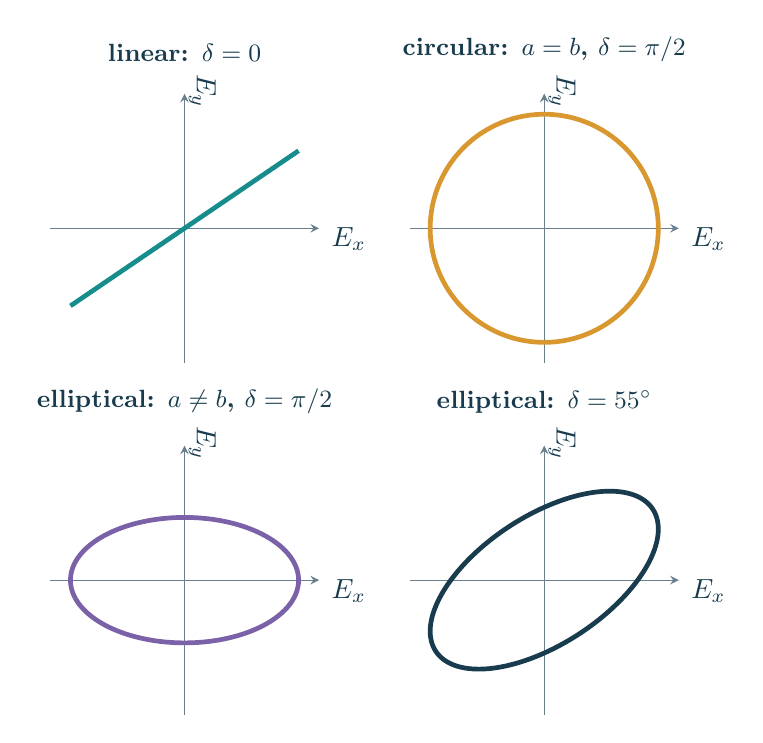
\begin{tikzpicture}[font=\sffamily]
\begin{groupplot}[
  group style={group size=2 by 2,horizontal sep=1.15cm,vertical sep=1.05cm},
  width=5.25cm,height=5.0cm,
  axis equal image,
  xmin=-1.18,xmax=1.18,ymin=-1.18,ymax=1.18,
  axis lines=middle,
  axis line style={ink!65,-stealth},
  ticks=none,
  xlabel={$E_x$},ylabel={$E_y$},
  xlabel style={at={(axis description cs:1.01,.46)},anchor=west,ink},
  ylabel style={at={(axis description cs:.48,1.01)},anchor=south,rotate=-90,ink},
  title style={ink,font=\small\bfseries,yshift=2pt}
]
\nextgroupplot[title={linear: $\delta=0$}]
  \addplot[teal,line width=1.7pt,domain=0:360,samples=361]
    ({cos(x)},{0.68*cos(x)});
\nextgroupplot[title={circular: $a=b$, $\delta=\pi/2$}]
  \addplot[gold,line width=1.7pt,domain=0:360,samples=361]
    ({cos(x)},{cos(x-90)});
\nextgroupplot[title={elliptical: $a\ne b$, $\delta=\pi/2$}]
  \addplot[violet,line width=1.7pt,domain=0:360,samples=361]
    ({cos(x)},{0.55*cos(x-90)});
\nextgroupplot[title={elliptical: $\delta=55^\circ$}]
  \addplot[ink,line width=1.7pt,domain=0:360,samples=361]
    ({cos(x)},{0.78*cos(x-55)});
\end{groupplot}
\end{tikzpicture}
\end{document}
